%!TEX root = ../../csuthesis_main.tex
\chapter{系统总体设计}

\section{系统架构设计}

本课题旨在基于 Carla 仿真平台构建一个集自动驾驶控制、视觉目标检测与跟踪、行为意图识别与可视化预警于一体的智能驾驶实验系统,支持对前方交通参与者(如车辆、行人)的持续感知与交互行为分析。系统整体采用模块化结构设计,确保各功能组件之间具有良好的可扩展性与独立性,适应未来算法优化与模型替换的需求。
本研究所设计的系统架构如图 3-1 所示,主要包含以下六个核心模块:

\textbf{仿真环境模块(Carla Simulator):}提供高精度虚拟城市道路、动态交通参与者、本车运动模型等仿真元素。通过 Carla 提供的 Python API 接口,系统可控制自动驾驶车辆在指定地图(Town10 和 Town01)中生成并实时运行,为后续感知与控制模块提供仿真数据输入。

\textbf{本车驾驶控制模块:}通过主控脚本 client\_bounding\_boxes.py的control(self, car) 函数实现,支持对仿真中自车的控制指令(加速、制动、转向等)输入,同时具备与传感器同步、车辆状态管理等功能。该模块为系统提供运行主循环与控制接口,其他子模块均挂载于此框架之上。

\textbf{图像采集与传感器模块:}使用 Carla 中的 RGB 摄像头传感器挂载于本车前部,用于采集每帧图像数据。采集结果通过回调机制传入主进程中,并进行图像渲染、保存与下游算法处理。摄像头配置参数(分辨率、视场角)可灵活调整,确保满足不同算法输入要求。

\textbf{目标检测与跟踪模块:}在系统中集成了 DeepSORT 实时多目标跟踪算法。每一帧图像经过外部目标检测器处理后,检测框与类别被输入到 DeepSORT 模型中,通过卡尔曼滤波与 ReID 特征关联机制实现目标的持续跟踪。系统当前以“选择最近目标”作为单目标策略,确保重点关注自车正前方可能构成威胁的对象。

\textbf{行为意图分析模块:}结合跟踪目标的相对位置、速度以及帧间距离变化,使用基于物理规则的方法对目标行为进行分类判断。该模块可识别目标是否“靠近”、“远离”或“危险接近”,并生成语义化标签。该功能设计轻量,不依赖深度模型,适用于实时反馈与交互控制。

\textbf{结果可视化与数据存储模块:}系统利用 Pygame 接口将每帧图像、边界框、跟踪 ID 与行为意图标签实时渲染至显示窗口。所有数据(图像 + 标签)每隔一定帧间隔自动存储至本地目录,用于后续模型训练或分析回放,具备良好的数据采集与复用能力。

\begin{figure}[H]
    \centering
    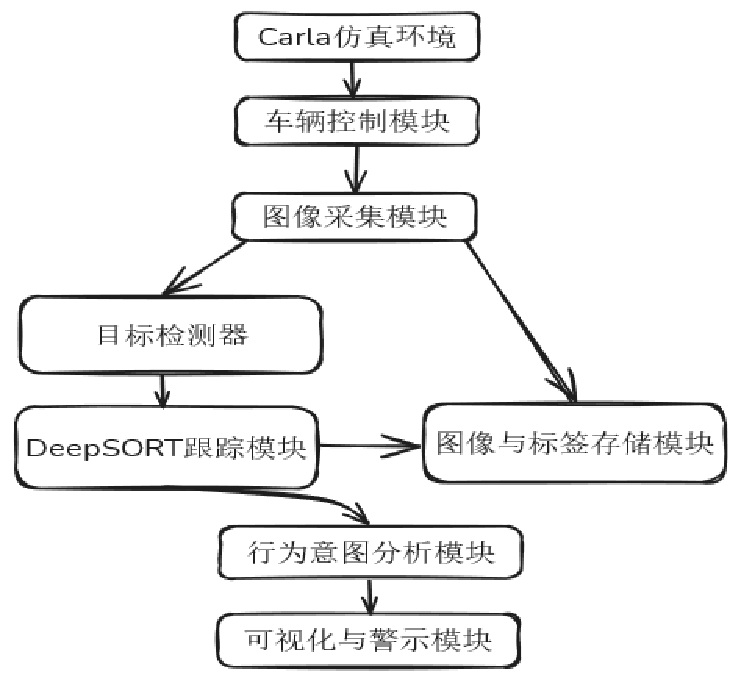
\includegraphics[width=0.8\textwidth]{images/图3 系统架构图.pdf}  % 引用转换后的 PDF 文件
    \caption{系统架构图}
    \label{fig:example_image}  % 可用于引用此图片
\end{figure}

\section{Carla 仿真平台与传感器配置}

为实现本课题中对自动驾驶车辆的控制、视觉感知与目标行为意图分析等功能,系统采用 Carla(Car Learning to Act)作为仿真平台,构建高度还原的城市交通环境。Carla 是由 Intel Labs 与 Computer Vision Center 联合开发的一款开源自动驾驶仿真平台,具备高保真度的城市地图、多种传感器模拟器、车辆物理引擎及交通流管理能力,广泛应用于自动驾驶研究领域。

\subsection{仿真地图选择与场景设定}

本系统选择 Carla 自带的两张典型城市地图:Town10HD 和 Town01 作为主要测试场景。

Town10HD 场景包含多车道城市道路、交通信号灯、交叉路口、障碍物遮挡、静态与动态交通参与者等复杂因素,适用于测试系统在高密度交通环境下的感知鲁棒性与行为分析准确性。

\begin{figure}[H]
    \centering
    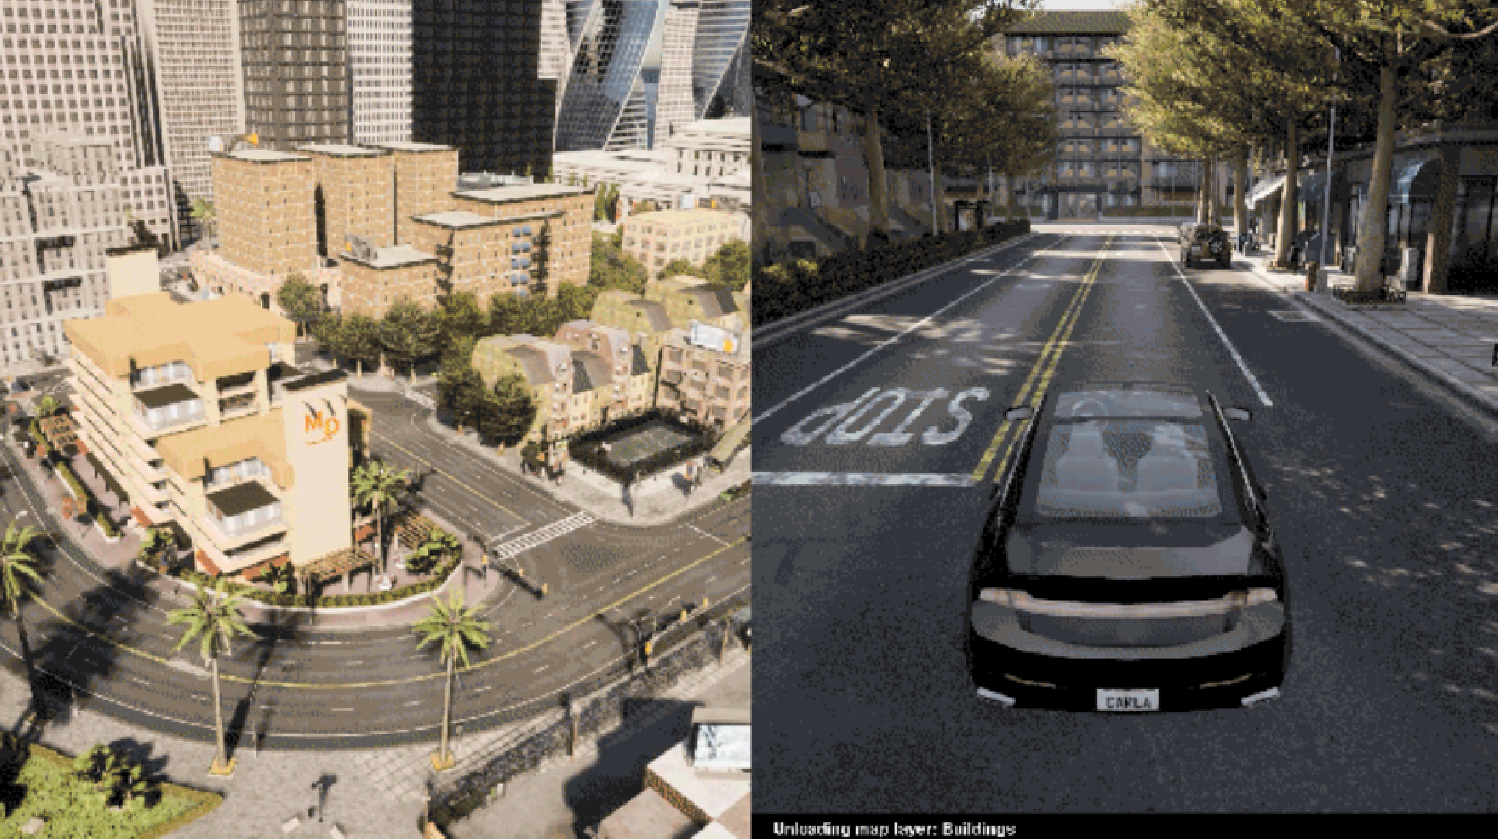
\includegraphics[width=0.8\textwidth]{images/图4 Town10HD地图展示.pdf}  % 引用转换后的 PDF 文件
    \caption{Town10HD地图展示}
    \label{fig:example_image}  % 可用于引用此图片
\end{figure}

Town01 场景则结构更为简单,适合用于算法功能验证与对比实验。

\begin{figure}[H]
    \centering
    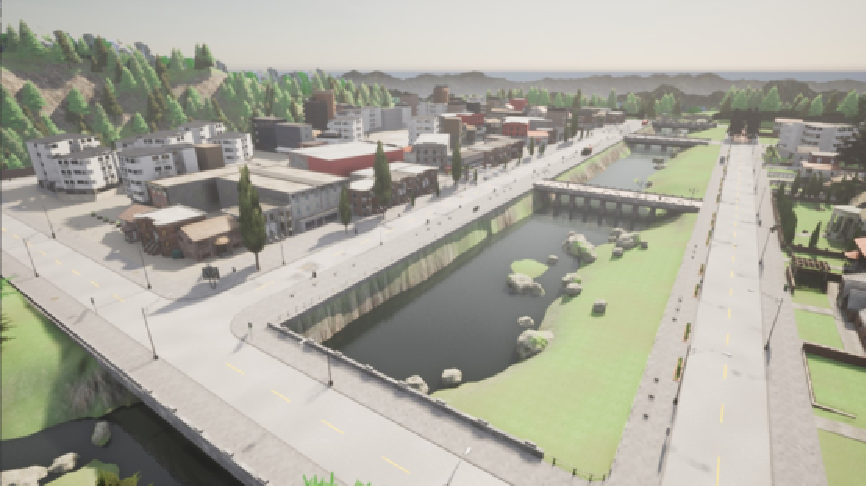
\includegraphics[width=0.8\textwidth]{images/图5 Town01地图展示.pdf}  % 引用转换后的 PDF 文件
    \caption{Town01地图展示}
    \label{fig:example_image}  % 可用于引用此图片
\end{figure}

仿真平台通过 Python API 方式加载地图并设置交通参与者生成密度与行为逻辑,确保每次启动后均可生成具有真实感的动态交通场景。

\subsection{本车模型与控制机制}

在系统初始化阶段,通过如下语句从 Carla 蓝图库中筛选车辆模型并生成本车:

\begin{figure}[H]
    \centering
    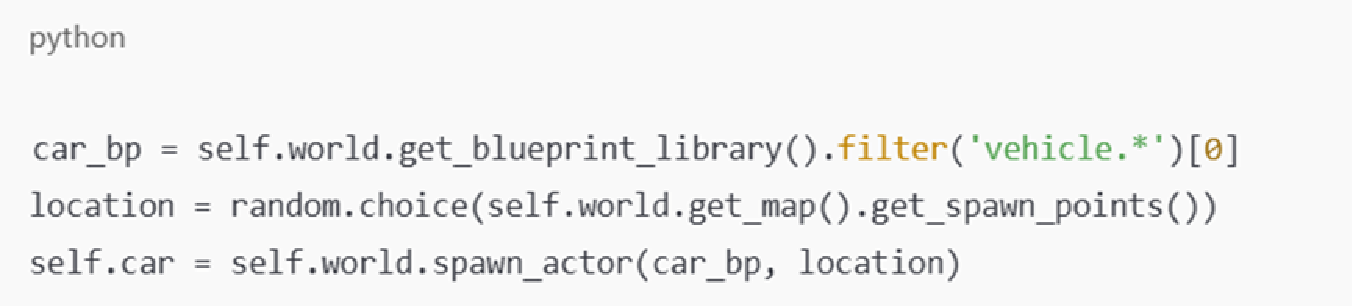
\includegraphics[width=0.8\textwidth]{images/图6 控制函数部分代码展示.pdf}  % 引用转换后的 PDF 文件
    \caption{控制函数部分代码展示}
    \label{fig:example_image}  % 可用于引用此图片
\end{figure}

车辆生成后系统对其施加控制命令,支持手动驾驶(通过键盘方向键操控)或接入后续自动控制模块。控制命令通过 Carla 的 car.apply\_control() 接口执行,包含油门、刹车、转向、手刹等基础控制量。

\subsection{摄像头传感器配置}
为获取车辆前方图像信息,系统在本车前部安装一个 RGB 摄像头传感器,其参数配置如下:
\begin{table}[htbp]
  \caption{摄像头参数配置表}
  \label{tab:camera_params}
  \centering
  \begin{tabular}{ll}
    \toprule
    参数 & 数值 \\
    \midrule
    分辨率 & 960 × 540(与系统窗口相适配) \\
    视场角(FOV) & 90° \\
    安装位置 & 自车后方5.5米,高度2.8米 \\
    俯仰角 & -15°,向下略俯视 \\
    \bottomrule
  \end{tabular}
\end{table}

摄像头配置由camera\_bp.set\_attribute()函数完成,采集的图像数据通过监听函数 self.camera.listen() 注册至主控循环,每帧图像均可进行目标检测、跟踪与意图分析,并实时渲染至用户界面或保存为数据集。

\subsection{其他配置说明}

为保证系统各模块对同一时刻图像帧的同步处理,本系统启用 Carla 的同步仿真模式(synchronous\_mode=True),确保每一步环境状态更新均与传感器输出一致,从而提升处理的可控性和图像帧稳定性。在同步模式下,系统以固定频率(20 FPS)调用 world.tick() 驱动环境演进,保证传感器输出与控制行为严格一一对应,有利于跟踪状态的正确匹配与分析逻辑的连续性。

此外,系统还通过 pygame 图形界面进行图像渲染,并使用 numpy、cv2、json 等工具库进行图像处理、数据标注与数据集构建操作。整体系统依赖 Carla Server 的标准运行(直接在 Windows 下双击启动 CarlaUE4.exe),确保模拟世界的稳定性与开放性。

\section{项目开发环境与工具链}

为高效实现自动驾驶场景下的视觉目标跟踪与意图识别算法,并完成系统级仿真测试与可视化功能开发,本文构建了一个基于 Carla 仿真平台的完整算法开发与测试环境。本节将对本项目使用的软硬件配置、开发语言、核心依赖库与工具链进行说明。

\subsection{开发硬件平台}

实验采用配置如下表的工作站,满足实时仿真需求:

\begin{table}[htbp]
  \caption{硬件配置表}
  \label{tab:hardware_config}
  \centering
  \begin{tabular}{ll}
    \toprule
    组件 & 规格 \\
    \midrule
    CPU & Intel Core i7-10750H @ 2.60GHz \\
    GPU & NVIDIA RTX 2060 (6GB GDDR6) \\
    内存 & 16GB DDR4 \\
    存储 & 512GB NVMe SSD \\
    \bottomrule
  \end{tabular}
\end{table}

\subsection{开发软件与工具}

项目开发主要在 Windows 10 平台下进行,核心依赖环境和工具包括:

\begin{table}[htbp]
  \caption{软件工具链配置}
  \label{tab:software_stack}
  \centering
  \begin{tabular}{lll}
    \toprule
    软件 & 版本 & 用途 \\
    \midrule
    Python & 3.7.9 & 主控程序开发 \\
    Carla & 0.9.15 & 自动驾驶仿真 \\
    Pygame & 2.5.2 & 可视化界面渲染与用户交互界面 \\
    OpenCV & 4.8.0 & 图像读取与保存,数据集采集处理 \\
    deep\_sort\_realtime & 1.3.2 & 多目标跟踪 \\
    \bottomrule
  \end{tabular}
\end{table}

其中,Carla Simulator 的安装与启动采取图形化模式:通过双击启动CarlaUE4.exe 打开仿真服务端,并在客户端代码运行过程中以 TCP 方式通信(默认端口 2000)。为了保障数据同步性,系统统一采用 Carla 的同步模式运行,确保传感器输出、车辆控制与仿真时间严格对齐。

Python 环境使用 Anaconda 管理,创建独立虚拟环境后通过 pip install 安装依赖库,确保版本稳定性与可复现性。部分库如 deep\_sort\_realtime 通过 PyPI 获取,或根据官方 GitHub 源码安装。




\begin{tabular}{l l}
%  \verb|\songti| & {\songti 宋体} \\
%  \verb|\heiti| & {\heiti 黑体} \\
%   \verb|\kaiti| & {\kaiti 楷体}
\end{tabular}
